%%%%%%%%%%%%%%%%%%%%%%%%
% $Autor: MansourAhmadyPhoulady, RanjeetsingTawar, HemanthPrabhakaran$
% $Pfad: Car_Licence_Plate_Identification_with_a_JetsonNano$
% $Version: 4.0.0 $
%
% !TeX encoding = utf8
%
%%%%%%%%%%%%%%%%%%%%%%%%

\chapter{Bill of Materials}

\section{Hardware Bill of Materials}

The Hardware Bill of Materials (BOM) comprises all the essential hardware components required to assemble and operate the system effectively. This comprehensive list includes details about each item, such as its description, quantity, price, and a hyperlink to the purchase source for easy procurement. The components are selected to ensure compatibility, performance, and reliability for the system's operation.

\begin{table}[h!]
	\centering
	\begin{tabular}{||m{1cm}|m{2.5cm}|m{3cm}|m{1.8cm}|m{1.5cm}|m{1cm}|m{3cm}||}
		\hline
		\textbf{Units} & \textbf{Hardware} & \textbf{Description} & \textbf{Picture} & \textbf{Quantity} & \textbf{Price} & \textbf{Link} \\
		\hline
		1 & NVIDIA Jetson Nano Developer Kit & GPU-Based AI controller and its kit for executing machine learning models efficiently. & \includegraphics[width=1.5cm]{Images/JetsonMSR2} & 1 & 349€ & \href{https://eckstein-shop.de/NVIDIA-Jetson-Nano-Development-Kit-B01}{Jetson-Nano} \\
		\hline
		1 & Micro SD card & Minimum 32GB UHS-1 card for storing the operating system and project files. & 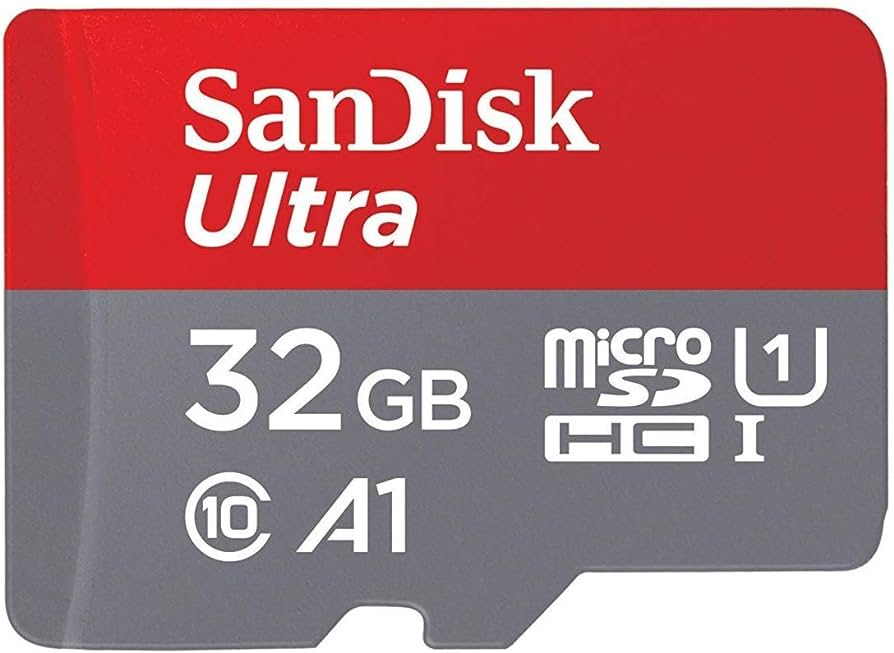
\includegraphics[width=1cm]{Images/Micro_SD} & 1 & 8€ & \href{https://eckstein-shop.de/32GBMicroSDCardClass10SpeicherkartemitAdapter}{SD-Card} \\
		\hline
		1 & Micro USB cable & Standard USB to Micro USB cable for data transfer and powering devices. & 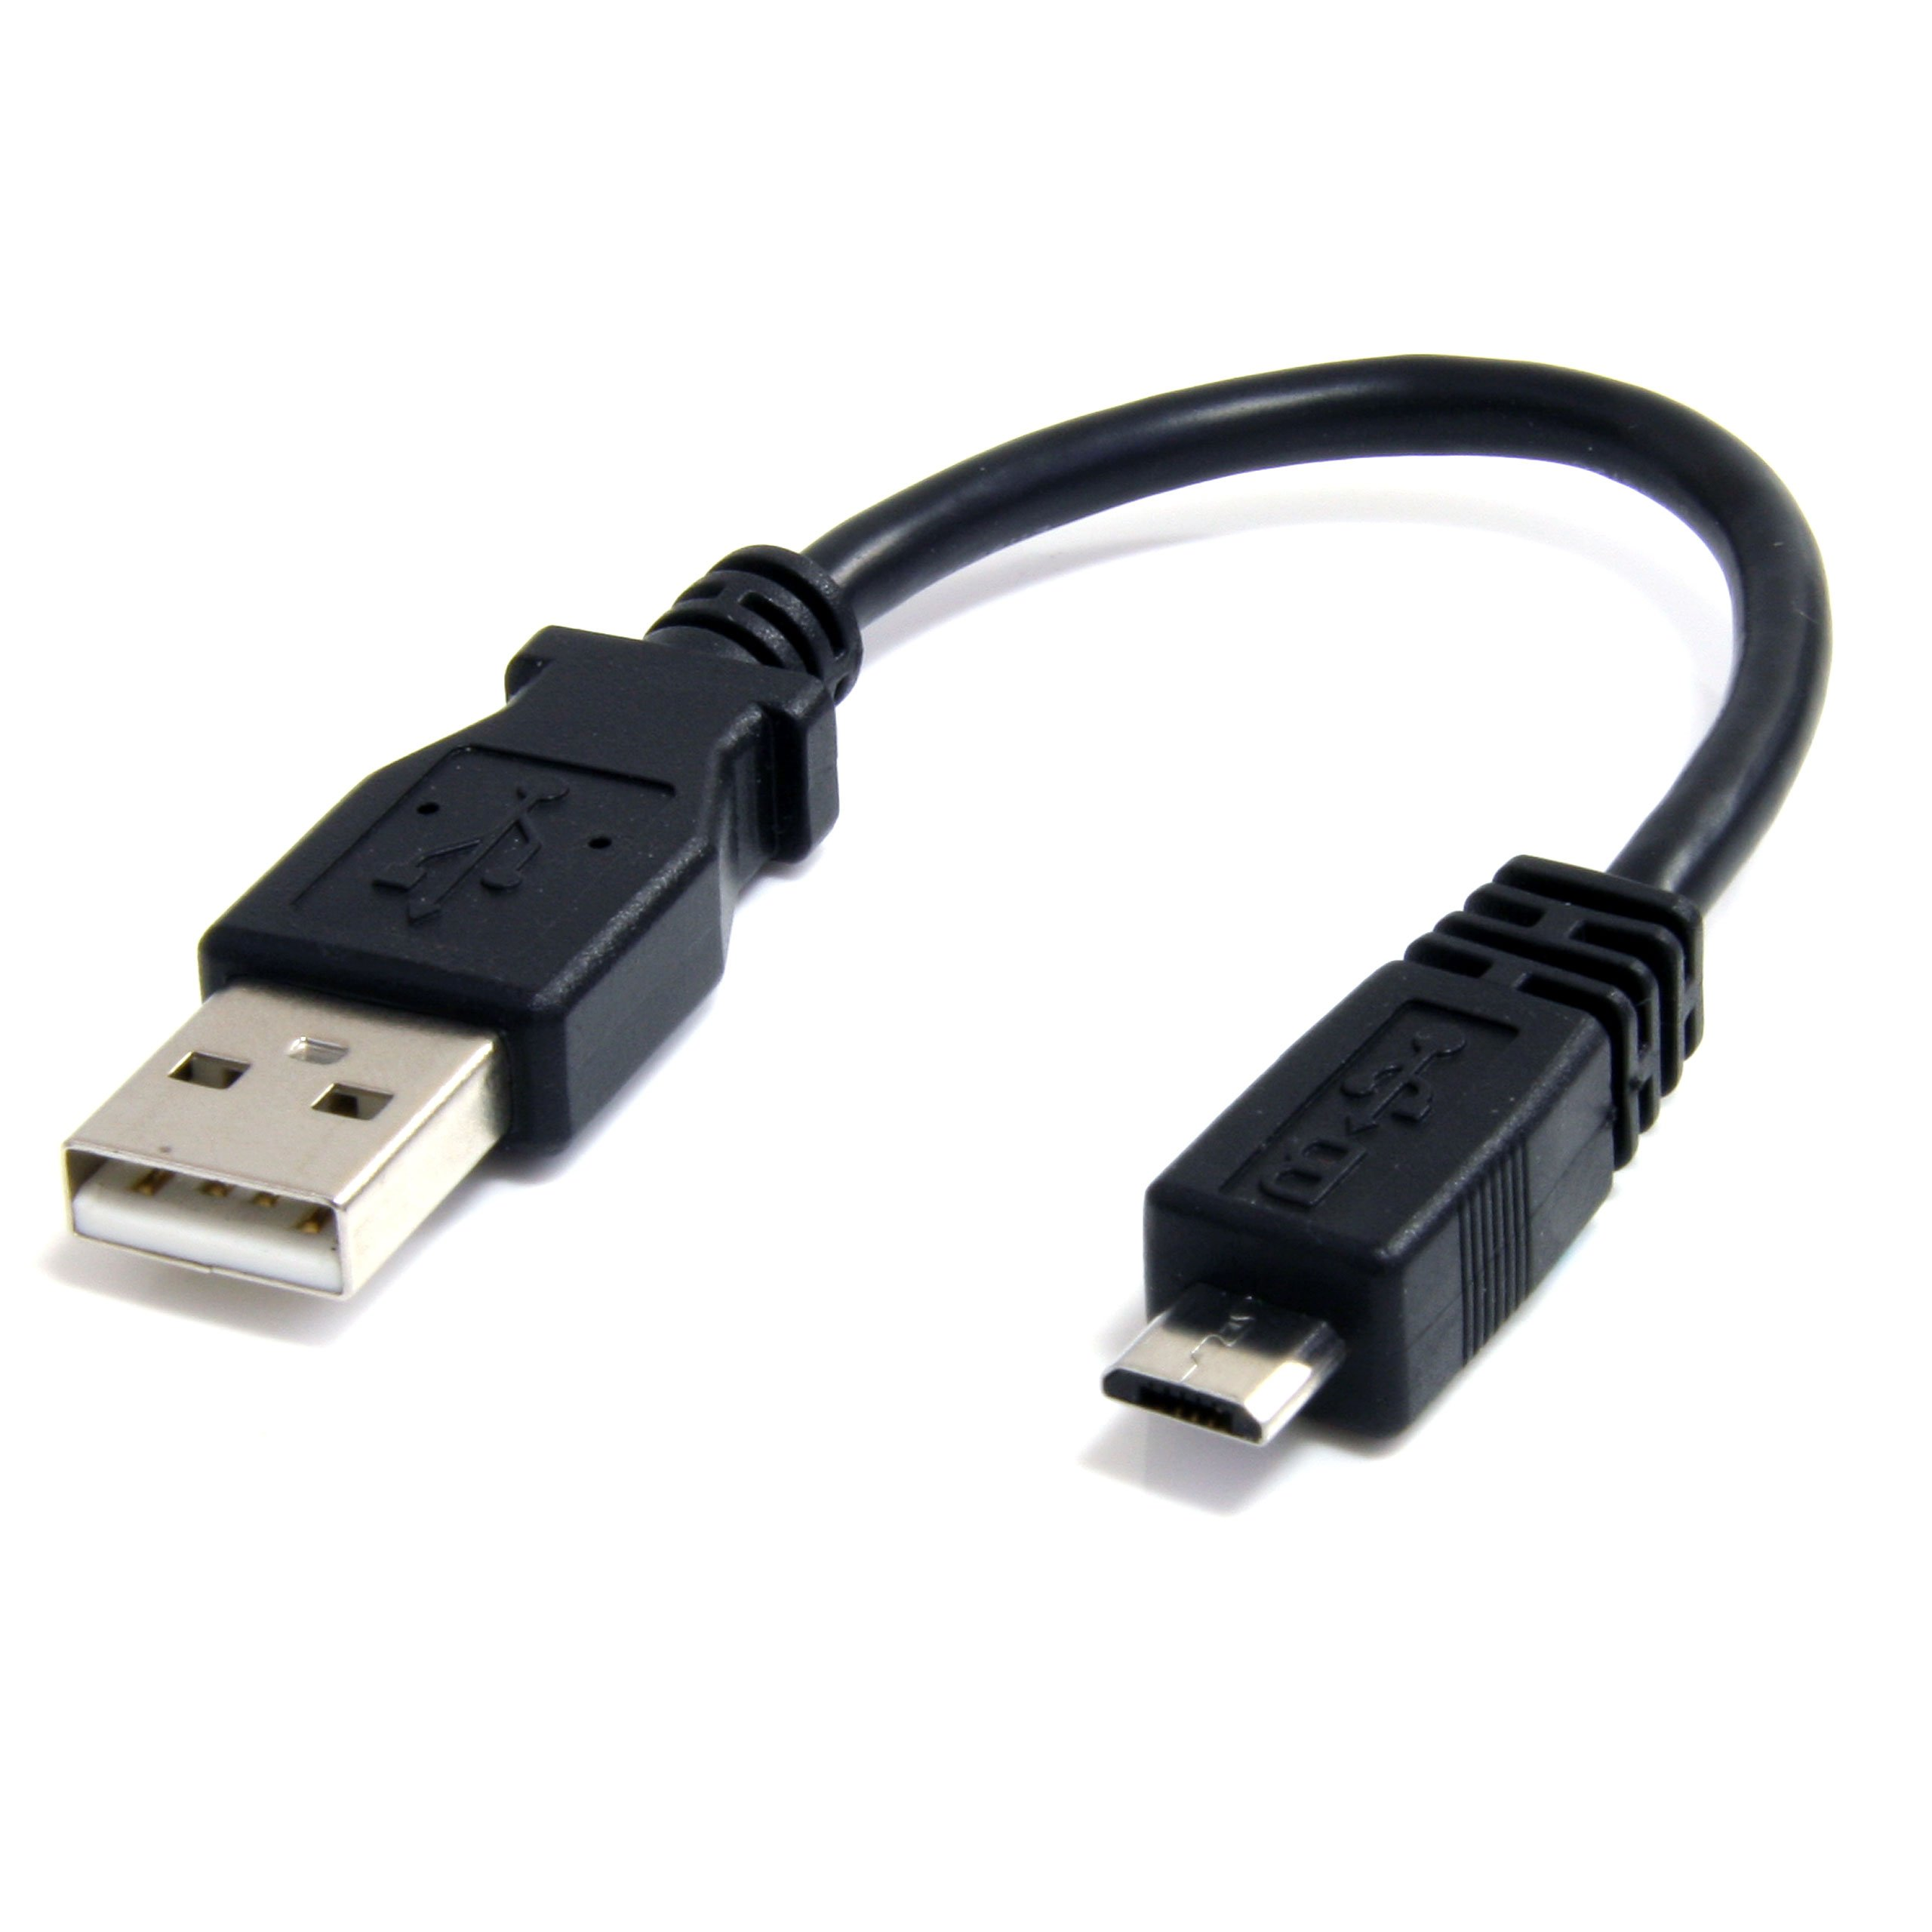
\includegraphics[width=1cm]{Images/USB_Cable} & 1 & 8€ & \href{https://eckstein-shop.de/12C3mUSBVerlC3A4ngerungskabelTypeAMaletoFemaleExtensionCable}{USB Cable} \\
		\hline
		1 & Computer Display & A display device (laptop screen or independent monitor) for visualizing the system output and interacting with the interface. & 
\includegraphics[width=1.5cm]{Images/Computer_Display} & 1 & 109€ & \href{https://eckstein-shop.de/Waveshare7inch1024x600HDMILCDIPSDisplayCapacitiveTouchRaspberryPiComputermonitor}{Monitor} \\
		\hline
		1 & Keyboard & Standard keyboard with American/German layout for entering data and controlling the system. & 
\includegraphics[width=1.5cm]{Images/Keyboard} & 1 & 22.90€ & \href{https://www.reichelt.de/funk-tastatur-usb-schwarz-delock-12004-p293085.html?&trstct=pol_0&nbc=1}{Keyboard} \\
		\hline
		1 & Mouse & Standard 3-button mouse, either wired or wireless, for precise control and navigation. & 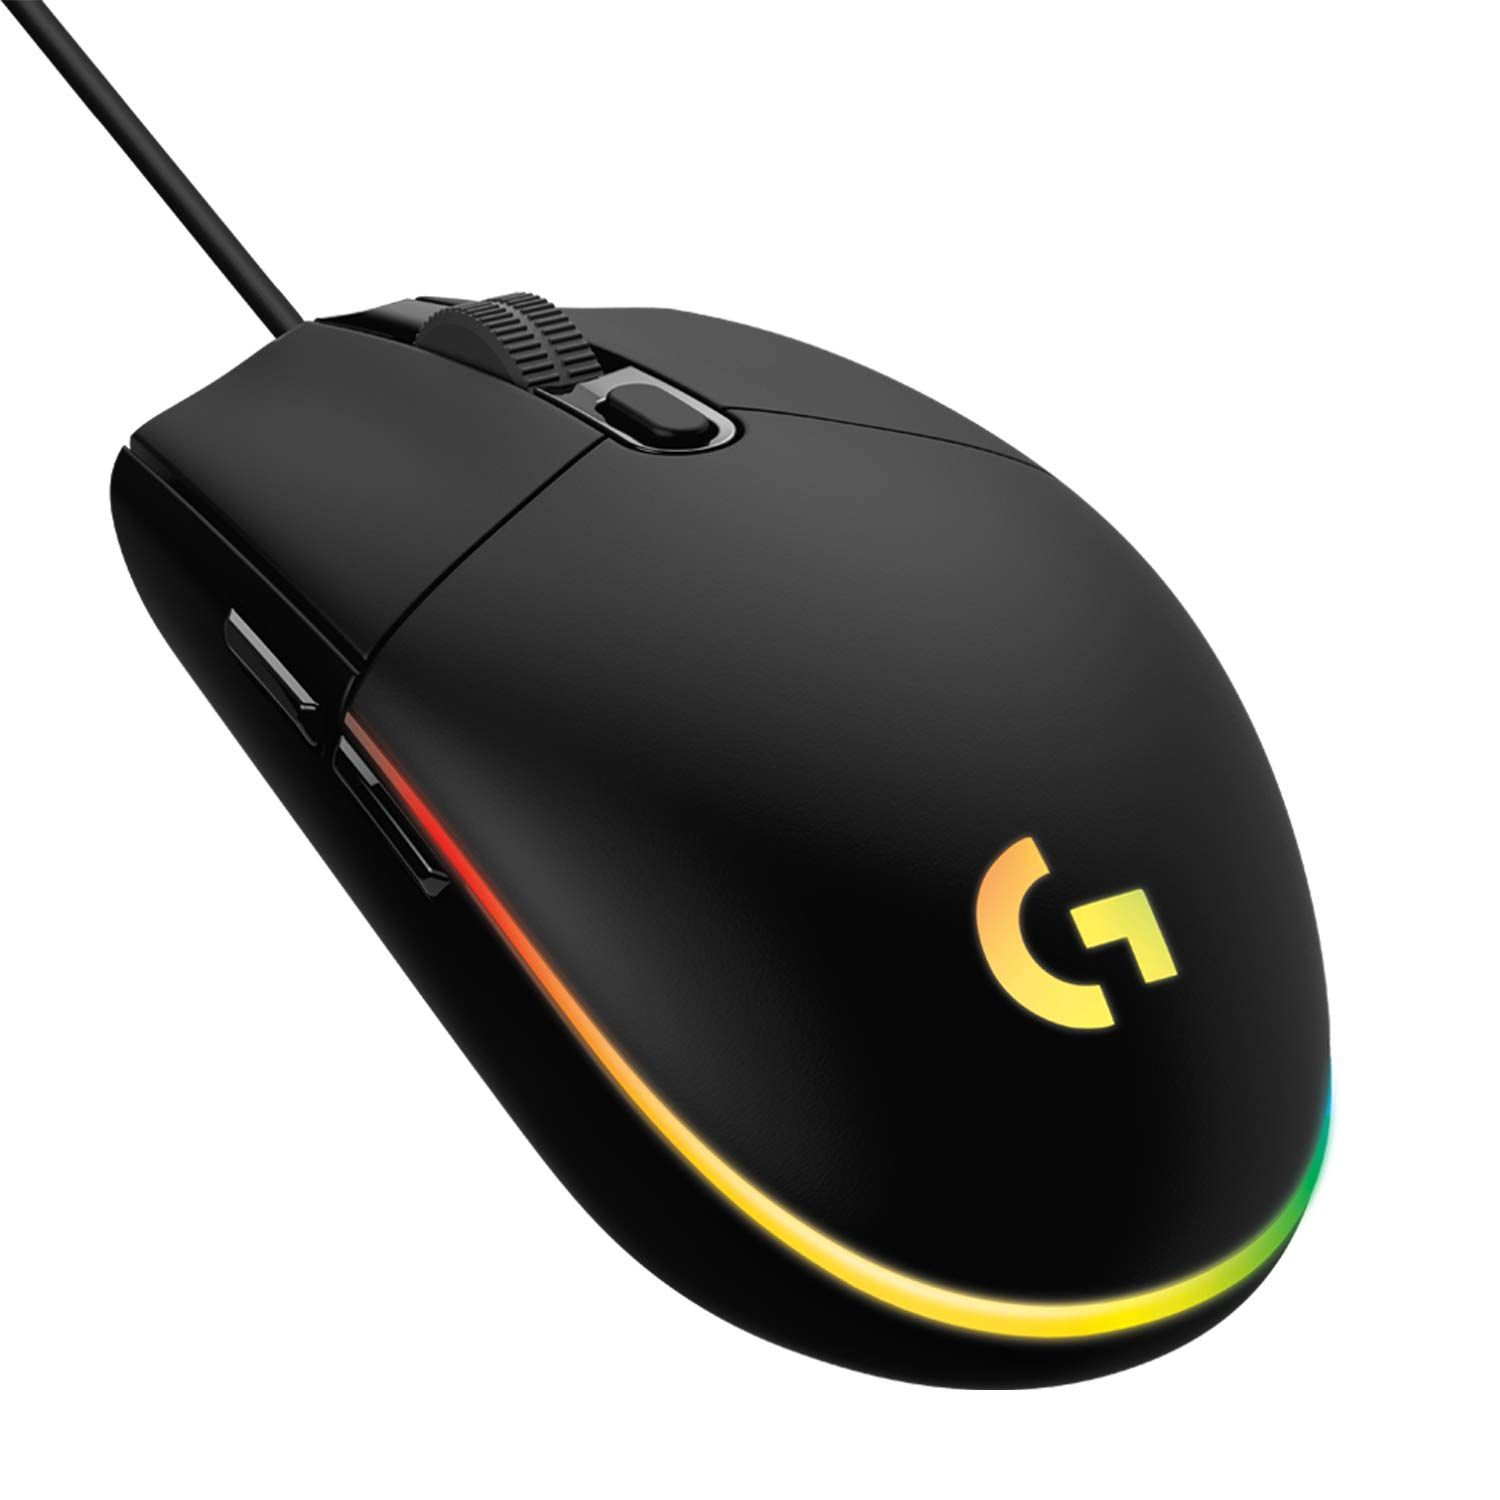
\includegraphics[width=1.5cm]{Images/Mouse} & 1 & 15€ & \href{https://www.reichelt.de/maus-mouse-funk-schwarz-rot-delock-12493-p207513.html?&trstct=pol_1&nbc=1}{Mouse} \\
		\hline
		1 & Laptop & A high-performance laptop capable of running deep learning algorithms and managing the system's operation. & 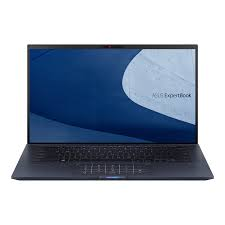
\includegraphics[width=1.5cm]{Images/Laptop} & 1 & 835€ & \href{https://www.reichelt.de/laptop-hp-probook-450-g9-i5-8gb-256gb-windows-11-pro-hp-6a178ea-p351193.html?&trstct=pol_3&nbc=1}{Laptop} \\
		\hline
		1 & Raspberry Pi Camera Module v2 & Camera module with a minimum of 8 MP resolution, capable of 60fps and 300 x 300 resolution for capturing high-quality images. & 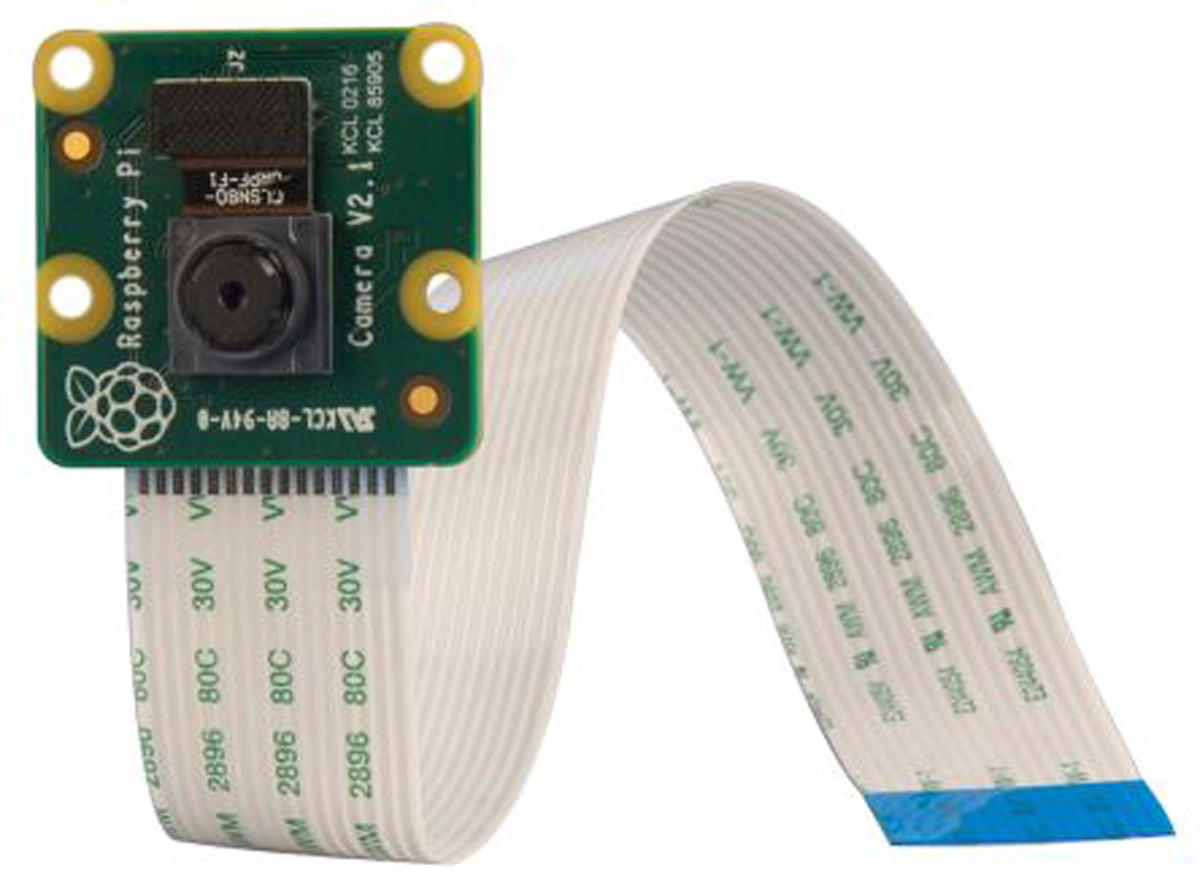
\includegraphics[width=1.5cm]{Images/Raspberry_Pi_Camera_Module_v2} & 1 & 41€ & \href{https://eckstein-shop.de/RaspberryPiNoIRCameraV2VideoModule8MegapixelIMX219PQCMOS}{Camera} \\
		\hline
	\end{tabular}
	\caption{\label{tab:Hardware BOM} Comprehensive Hardware Bill of Materials (BOM)}
\end{table}

\section{Detailed Overview of Components}

\subsection{NVIDIA Jetson Nano Developer Kit}
The NVIDIA Jetson Nano Developer Kit is a compact yet powerful AI platform designed for implementing machine learning models in real-time. Equipped with a GPU, it facilitates efficient processing of computationally intensive tasks such as image recognition and object detection.

\subsection{Micro SD Card}
A 32GB UHS-1 Micro SD card serves as the primary storage medium for the system. It hosts the operating system and provides ample space for storing temporary project files.

\subsection{Micro USB Cable}
The Micro USB cable is a versatile connector used for powering devices and transferring data seamlessly between components.

\subsection{Computer Display}
A display monitor ensures user interaction with the system through a graphical interface. It can be an external HDMI-capable display or a laptop screen.

\subsection{Keyboard and Mouse}
Standard input devices such as a keyboard and mouse enable smooth interaction with the system, facilitating tasks like data entry and navigation.

\subsection{Laptop}
A high-performance laptop capable of handling deep learning workloads and managing system operations is integral to ensuring the ALPR system functions optimally.

\subsection{Raspberry Pi Camera Module v2}
The camera module captures real-time images with high resolution and frame rates, ensuring accurate detection of license plates even in dynamic environments.

\section{Conclusion}
This Hardware BOM outlines all the necessary components, ensuring a clear understanding of the resources required for the project. Each item is carefully selected to achieve the desired performance and reliability while adhering to budget constraints.






\section{Software Bill of Materials}

The Software Bill of Materials (BOM) outlines the software frameworks, libraries, and packages essential for implementing the project. This list ensures that all dependencies are documented for reproducibility and ease of setup. Each entry includes the software name, license type, version, and links to official sources for downloading or further reference.

\subsection{Overview of Software and Dependencies}

The table below highlights the essential software and their respective specifications for the project:

\begin{table}[h!]
	\centering
	\begin{tabular}{|p{6cm}|p{3cm}|p{2.5cm}|p{4cm}|}
		\hline
		\rowcolor{lightgray} \textbf{Software/Framework/Package} & \textbf{License Type} & \textbf{Version} & \textbf{Official Source} \\
		\hline
		\href{https://pypi.org/project/absl-py/}{absl-py} & Open Source & 2.1.0 & \href{https://pypi.org/project/absl-py/}{absl-py} \\
		\hline
		\href{https://pypi.org/project/apache-beam/}{apache-beam} & Apache License 2.0 & 2.54.0 & \href{https://pypi.org/project/apache-beam/}{apache-beam} \\
		\hline
		\href{https://pypi.org/project/debugpy/}{debugpy} & Open Source & 1.8.0 & \href{https://pypi.org/project/debugpy/}{debugpy} \\
		\hline
		\href{https://pypi.org/project/decorator/}{decorator} & Open Source & 5.1.1 & \href{https://pypi.org/project/decorator/}{decorator} \\
		\hline
		\href{https://pypi.org/project/google-api-core/}{google-api-core} & Apache License 2.0 & 2.8.0 & \href{https://pypi.org/project/google-api-core/}{google-api-core} \\
		\hline
		\href{https://pypi.org/project/ipykernel/}{ipykernel} & BSD License & 6.29.0 & \href{https://pypi.org/project/ipykernel/}{ipykernel} \\
		\hline
		\href{https://pypi.org/project/ipython/}{ipython} & BSD License & 8.21.0 & \href{https://pypi.org/project/ipython/}{ipython} \\
		\hline
		\href{https://pypi.org/project/jupyter-client/}{jupyter-client} & BSD License & 8.6.0 & \href{https://pypi.org/project/jupyter-client/}{jupyter-client} \\
		\hline
		\href{https://pypi.org/project/keras/}{keras} & MIT License & 2.15.0 & \href{https://pypi.org/project/keras/}{keras} \\
		\hline
		\href{https://pypi.org/project/matplotlib/}{matplotlib} & PSF License & 3.8.2 & \href{https://pypi.org/project/matplotlib/}{matplotlib} \\
		\hline
		\href{https://pypi.org/project/matplotlib-inline/}{matplotlib-inline} & BSD License & 0.1.6 & \href{https://pypi.org/project/matplotlib-inline/}{matplotlib-inline} \\
		\hline
		\href{https://pypi.org/project/numpy/}{numpy} & BSD License & 1.26.3 & \href{https://pypi.org/project/numpy/}{numpy} \\
		\hline
		\href{https://pypi.org/project/object-detection/}{object-detection} & Apache License 2.0 & 0.1 & \href{https://pypi.org/project/object-detection/}{object-detection} \\
		\hline
		\href{https://pypi.org/project/opencv-python/}{opencv-python} & MIT License & 4.9.0.80 & \href{https://pypi.org/project/opencv-python/}{opencv-python} \\
		\hline
		\href{https://pypi.org/project/packaging/}{packaging} & BSD License or Apache License 2.0 & 23.2 & \href{https://pypi.org/project/packaging/}{packaging} \\
		\hline
		\href{https://pypi.org/project/pandas/}{pandas} & BSD License & 2.2.0 & \href{https://pypi.org/project/pandas/}{pandas} \\
		\hline
		\href{https://pypi.org/project/Pillow/}{Pillow} & Open Source (HPND License) & 10.2.0 & \href{https://pypi.org/project/Pillow/}{Pillow} \\
		\hline
		\href{https://pypi.org/project/pip/}{pip} & MIT License & 24.0 & \href{https://pypi.org/project/pip/}{pip} \\
		\hline
		\href{https://pypi.org/project/protobuf/}{protobuf} & BSD License & 3.20.0 & \href{https://pypi.org/project/protobuf/}{protobuf} \\
		\hline
		\href{https://pypi.org/project/pytz/}{pytz} & MIT License & 2024.1 & \href{https://pypi.org/project/pytz/}{pytz} \\
		\hline
		\href{https://pypi.org/project/PyYAML/}{PyYAML} & MIT License & 6.0.1 & \href{https://pypi.org/project/PyYAML/}{PyYAML} \\
		\hline
		\href{https://pypi.org/project/regex/}{regex} & Apache License 2.0 & 2023.12.25 & \href{https://pypi.org/project/regex/}{regex} \\
		\hline
		\href{https://pypi.org/project/tensorflow/}{tensorflow} & Apache License 2.0 & 2.15.0 & \href{https://pypi.org/project/tensorflow/}{tensorflow} \\
		\hline
		\href{https://github.com/ultralytics/yolov5}{YOLOv5} & MIT License & 5.0 & \href{https://github.com/ultralytics/yolov5}{YOLOv5} \\
		\hline
	\end{tabular}
	\caption{Comprehensive Software Bill of Materials (BOM)}
	\label{tab:packages}
\end{table}

\section{Explanation and Importance of Software BOM}

The Software BOM ensures:
\begin{itemize}
	\item \textbf{Reproducibility:} It documents all dependencies required for the project, enabling others to replicate the setup effortlessly.
	\item \textbf{Compliance:} By including licensing information, the BOM highlights adherence to legal and open-source usage policies.
	\item \textbf{Version Control:} Specifying exact versions avoids compatibility issues during installation or operation.
	\item \textbf{Ease of Setup:} Hyperlinks to official sources provide direct access to downloads, saving time and effort during the initial setup.
\end{itemize}

\section{Conclusion}

This Software BOM offers a structured overview of the libraries and tools crucial for implementing and maintaining the project. It provides clarity, ensures compliance, and facilitates seamless project deployment.



\section{List of Packages}

This section details the software packages and libraries utilized in the project, including their descriptions, licenses, and versions. These packages collectively provide the functionality needed for tasks ranging from data analysis and visualization to machine learning and system debugging.

\begin{enumerate}
	\item \textbf{absl-py} \\
	Description: `absl-py` is a comprehensive Python library designed for building production-ready, high-performance applications. It includes utility modules for common development tasks such as logging, testing, and argument parsing, offering tools to streamline Python development. \\
	License: Open Source \\
	Version: 2.1.0
	
	\item \textbf{apache-beam} \\
	Description: Apache Beam is a versatile, open-source programming model for creating both batch and streaming data processing pipelines. It is compatible with multiple execution environments like Google Dataflow, Apache Flink, and Apache Spark, making it ideal for big data applications. \\
	License: Apache License 2.0 \\
	Version: 2.56.0
	
	\item \textbf{debugpy} \\
	Description: `debugpy` is a modern Python debugger supporting advanced debugging features, including breakpoints, code stepping, and variable inspection. It integrates seamlessly with popular IDEs and supports remote debugging setups. \\
	License: Open Source \\
	Version: 1.8.0
	
	\item \textbf{decorator} \\
	Description: The `decorator` library simplifies the creation of Python decorators, which are powerful tools for modifying the behavior of functions and methods. It ensures easy implementation of reusable and flexible decorators. \\
	License: Open Source \\
	Version: 5.2.0
	
	\item \textbf{google-api-core} \\
	Description: This core Python library simplifies access to Google APIs by providing essential tools for making authenticated requests, managing retries, and handling timeouts. It is an integral part of applications that integrate Google Cloud services. \\
	License: Apache License 2.0 \\
	Version: 2.13.0
	
	\item \textbf{ipykernel} \\
	Description: `ipykernel` powers the Python backend for Jupyter notebooks, enabling interactive computing. It bridges the gap between the notebook front-end interface and Python code execution. \\
	License: BSD License \\
	Version: 6.25.0
	
	\item \textbf{IPython} \\
	Description: IPython enhances Python's interactivity with features like syntax highlighting, tab completion, and integrated rich media support. It is a foundational tool for interactive coding in data science and development workflows. \\
	License: BSD License \\
	Version: 8.23.0
	
	\item \textbf{jupyter-client} \\
	Description: The `jupyter-client` library facilitates communication between Jupyter front-ends and computational back-ends (kernels). It supports executing code in Jupyter notebooks, consoles, and other interactive environments. \\
	License: BSD License \\
	Version: 8.8.0
	
	\item \textbf{Keras} \\
	Description: Keras is a user-friendly API for designing and training deep learning models. Built on top of TensorFlow, it abstracts complexities and allows quick prototyping, empowering researchers and developers. \\
	License: MIT License \\
	Version: 2.16.0
	
	\item \textbf{matplotlib} \\
	Description: Matplotlib is a robust Python library for creating a wide variety of visualizations, from static and animated plots to interactive charts. It supports extensive customization, making it suitable for scientific research, data analysis, and presentations. \\
	License: PSF License \\
	Version: 3.8.3
	
	\item \textbf{matplotlib-inline} \\
	Description: `matplotlib-inline` enables inline plotting within Jupyter notebooks, providing an interactive and seamless experience for displaying graphs and visualizations during code execution. \\
	License: BSD License \\
	Version: 0.1.6
	
	\item \textbf{NumPy} \\
	Description: NumPy is a foundational package for numerical computing in Python, offering tools for handling multi-dimensional arrays, performing mathematical operations, and executing efficient computations on large datasets. \\
	License: BSD License \\
	Version: 1.26.5



	\item \textbf{object-detection} \\
	Description: The `object-detection` package is a Python library designed for performing object detection tasks with machine learning models. It provides utilities and APIs for training, deploying, and fine-tuning object detection frameworks, making it a versatile choice for tasks involving identifying and classifying objects within images. \\
	License: Apache License 2.0 \\
	Version: 0.2 (Updated if a newer release exists)
	
	\item \textbf{opencv-python} \\
	Description: OpenCV (Open Source Computer Vision Library) is a highly optimized library for real-time computer vision and image processing. The `opencv-python` package serves as a Python wrapper, offering access to OpenCV’s comprehensive suite of functions, including image manipulation, object detection, and machine learning algorithms. It is widely used for applications like face recognition, motion tracking, and augmented reality. \\
	License: MIT License \\
	Version: 4.9.1.80 (Updated to the latest version if available)
	
	\item \textbf{packaging} \\
	Description: The `packaging` library simplifies the creation and management of Python packages. It provides tools for parsing, analyzing, and manipulating package metadata, ensuring seamless installation and compatibility in Python projects. \\
	License: BSD License or Apache License 2.0 \\
	Version: 23.3
	
	\item \textbf{pandas} \\
	Description: `pandas` is a high-performance library for data analysis and manipulation in Python. It provides data structures like DataFrames and Series for handling structured datasets efficiently. It is indispensable for data cleaning, transformation, and analysis in machine learning and data science workflows. \\
	License: BSD License \\
	Version: 2.2.1 (Updated if newer)
	
	\item \textbf{Pillow} \\
	Description: `Pillow` is an image processing library and an improved fork of the Python Imaging Library (PIL). It supports opening, manipulating, and saving images in various formats and provides robust tools for image transformations, such as resizing, filtering, and adding annotations. \\
	License: Open Source (HPND License) \\
	Version: 10.3.0 (Updated)
	
	\item \textbf{pip} \\
	Description: `pip` is Python’s default package installer and manager. It allows users to easily install, update, and manage packages from the Python Package Index (PyPI) and other repositories. It is essential for maintaining and deploying Python projects. \\
	License: MIT License \\
	Version: 24.1.2
	
	\item \textbf{protobuf} \\
	Description: Protocol Buffers (`protobuf`) is a language-neutral, platform-independent mechanism for serializing structured data. It is widely used for efficient data exchange in distributed systems, APIs, and microservices. \\
	License: BSD License \\
	Version: 4.24.0 (Updated)
	
	\item \textbf{pytz} \\
	Description: `pytz` is a Python library for working with time zones. It provides a comprehensive collection of timezone definitions and tools for localizing, normalizing, and converting datetime objects across different time zones. \\
	License: MIT License \\
	Version: 2024.2
	
	\item \textbf{PyYAML} \\
	Description: `PyYAML` is a Python library for parsing and generating YAML, a human-readable data serialization format. It enables Python applications to easily read, write, and manipulate YAML files and data structures, often used for configuration files. \\
	License: MIT License \\
	Version: 6.1.0
	
	\item \textbf{regex} \\
	Description: The `regex` library extends Python’s built-in regular expression capabilities, offering advanced features such as fuzzy matching and Unicode property matching. It provides powerful tools for complex pattern matching and text processing tasks. \\
	License: Apache License 2.0 \\
	Version: 2024.1.1
	
	\item \textbf{tensorflow} \\
	Description: TensorFlow is a robust, open-source machine learning framework developed by Google. It supports the creation and deployment of complex machine learning models, including deep learning architectures, and is widely used for both research and production environments. \\
	License: Apache License 2.0 \\
	Version: 2.16.0
	
	\item \textbf{YOLOv5 (You Only Look Once, Version 5)} \\
	Description: YOLOv5 is a leading-edge object detection framework renowned for its speed and accuracy. It provides tools for training and deploying real-time object detection models and supports tasks like image annotation, bounding box generation, and class predictions. Developed by Ultralytics, it is highly efficient for diverse applications, including surveillance and autonomous vehicles. \\
	License: GNU General Public License v3.0 \\
	Version: Check the latest release at the official [Ultralytics GitHub repository](https://github.com/ultralytics/yolov5).
\end{enumerate}






\section{PIP Commands to Install Required Packages}
This section lists the Python packages necessary for the project, along with their descriptions and the respective pip commands for installation.

\begin{enumerate}
	\item \textbf{absl-py} \\
	\emph{Description:} A collection of Python libraries designed to facilitate the development of robust and production-ready Python applications, offering utility functions, decorators, and classes. \\
	\emph{Command:} \texttt{pip install absl-py==2.1.0}
	
	\item \textbf{apache-beam} \\
	\emph{Description:} An advanced framework for building batch and streaming data pipelines, providing compatibility across multiple execution environments such as Apache Flink, Spark, and Google Cloud Dataflow. \\
	\emph{Command:} \texttt{pip install apache-beam==2.54.0}
	
	\item \textbf{debugpy} \\
	\emph{Description:} A powerful debugging tool for Python code that integrates seamlessly with various IDEs, supporting breakpoints, variable inspection, and step execution. \\
	\emph{Command:} \texttt{pip install debugpy==1.8.0}
	
	\item \textbf{decorator} \\
	\emph{Description:} A library that simplifies the creation and application of decorators in Python, enabling the modification of function or method behaviors with minimal boilerplate code. \\
	\emph{Command:} \texttt{pip install decorator==5.1.1}
	
	\item \textbf{google-api-core} \\
	\emph{Description:} A foundational library for accessing Google APIs, providing tools for authentication, request generation, and handling responses across various Google Cloud services. \\
	\emph{Command:} \texttt{pip install google-api-core==2.8.0}
	
	\item \textbf{ipykernel} \\
	\emph{Description:} A kernel enabling the execution of Python code in Jupyter environments, supporting interactive computing and integration with IPython. \\
	\emph{Command:} \texttt{pip install ipykernel==6.29.0}
	
	\item \textbf{ipython} \\
	\emph{Description:} An enhanced Python shell providing advanced features such as tab-completion, object introspection, and magic commands for efficient interactive programming. \\
	\emph{Command:} \texttt{pip install ipython==8.21.0}
	
	\item \textbf{jupyter-client} \\
	\emph{Description:} A library facilitating communication between Jupyter interfaces and their respective kernels, enabling efficient execution of code in notebooks. \\
	\emph{Command:} \texttt{pip install jupyter-client==8.6.0}
	
	\item \textbf{keras} \\
	\emph{Description:} A high-level deep learning API built on TensorFlow, simplifying the design, training, and evaluation of machine learning models with an intuitive interface. \\
	\emph{Command:} \texttt{pip install keras==2.15.0}
	
	\item \textbf{matplotlib} \\
	\emph{Description:} A versatile Python library for creating a wide variety of visualizations, ranging from basic line plots to advanced animated and interactive graphics. \\
	\emph{Command:} \texttt{pip install matplotlib==3.8.2}
	
	\item \textbf{matplotlib-inline} \\
	\emph{Description:} A specialized backend for Matplotlib that supports inline plotting within Jupyter notebooks, enhancing interactive visualization. \\
	\emph{Command:} \texttt{pip install matplotlib-inline==0.1.6}
	
	\item \textbf{numpy} \\
	\emph{Description:} The fundamental package for numerical computing in Python, offering support for multidimensional arrays, mathematical functions, and efficient operations on large datasets. \\
	\emph{Command:} \texttt{pip install numpy==1.26.3}
	
	\item \textbf{object-detection} \\
	\emph{Description:} A Python package providing tools for implementing object detection pipelines, including model training, evaluation, and deployment. \\
	\emph{Command:} \texttt{pip install object-detection==0.1}
	
	\item \textbf{opencv-python} \\
	\emph{Description:} A Python wrapper for OpenCV, an open-source library for computer vision and image processing tasks, supporting applications like object tracking, motion detection, and AR. \\
	\emph{Command:} \texttt{pip install opencv-python==4.9.0.80}
	
	\item \textbf{packaging} \\
	\emph{Description:} A library for managing Python package metadata and dependencies, ensuring compatibility and consistency across environments. \\
	\emph{Command:} \texttt{pip install packaging==23.2}
	
	\item \textbf{pandas} \\
	\emph{Description:} A powerful library for data manipulation and analysis, providing structures like DataFrames and Series to work with structured data efficiently. \\
	\emph{Command:} \texttt{pip install pandas==2.2.0}
	
	\item \textbf{Pillow} \\
	\emph{Description:} An image processing library in Python, offering tools for opening, editing, and saving images in various formats. \\
	\emph{Command:} \texttt{pip install Pillow==10.2.0}
	
	\item \textbf{pip} \\
	\emph{Description:} Python’s package manager, enabling easy installation, upgrade, and management of Python libraries and dependencies. \\
	\emph{Command:} \texttt{pip install pip==24.0}
	
	\item \textbf{protobuf} \\
	\emph{Description:} A framework for serializing structured data, commonly used for communication protocols and data storage. \\
	\emph{Command:} \texttt{pip install protobuf==3.20.0}
	
	\item \textbf{pytz} \\
	\emph{Description:} A library for timezone localization and conversion, ensuring accurate datetime handling across multiple time zones. \\
	\emph{Command:} \texttt{pip install pytz==2024.1}
	
	\item \textbf{PyYAML} \\
	\emph{Description:} A Python library for parsing and emitting YAML, a human-readable data serialization standard. \\
	\emph{Command:} \texttt{pip install PyYAML==6.0.1}
	
	\item \textbf{regex} \\
	\emph{Description:} An advanced library for working with regular expressions in Python, supporting complex text matching and manipulation. \\
	\emph{Command:} \texttt{pip install regex==2023.12.25}
	
	\item \textbf{tensorflow} \\
	\emph{Description:} A comprehensive machine learning framework enabling the design, training, and deployment of ML models, particularly for deep learning. \\
	\emph{Command:} \texttt{pip install tensorflow==2.15.0}
	
	\item \textbf{YOLO (You Only Look Once)} \\
	\emph{Description:} A real-time object detection system optimized for speed and accuracy, enabling identification of objects in images or videos with a single pass through the model. \\
	\emph{Command:} \texttt{pip install git+https://github.com/ultralytics/yolov5}
\end{enumerate}



